\documentclass[twoside, 12pt, a4paper]{refart}
\usepackage[utf8]{inputenc}
\usepackage[russian]{babel}
\usepackage[T2A]{fontenc}
\usepackage{amsmath, amsfonts, amssymb, graphicx}
\usepackage{pscyr}
\usepackage{makeidx}
\usepackage{ifthen}
\usepackage{hyperref}
\hypersetup{colorlinks=true,linkcolor=blue,filecolor=magenta,urlcolor=blue}
\urlstyle{same}

\RequirePackage{caption}
\DeclareCaptionLabelSeparator{defffis}{ -- }
\captionsetup{justification=centering,labelsep=defffis}

\def\bs{\char'134 } % backslash in \tt font.
\newcommand{\ie}{i.\,e.,}
\newcommand{\eg}{e.\,g..}
\DeclareRobustCommand\cs[1]{\texttt{\char`\\#1}}

\title{Микрофлюидный контроллер давлений}
\author{
Автор настоящего руководства: \\
% Букатин Антон Сергеевич \\
Денисов Иван Андреевич \\
% Лукьяненко Кирилл Андреевич \\
% Сорокин Владимир Викторович \\
% Якимов Антон Сергеевич \\
Филатов Никита Алексеевич \\
}



\date{4 декабря 2019 г.}
\emergencystretch1em  %

\pagestyle{myfootings}
\markboth{Руководство: микрофлюидный контроллер давлений}%
         {Руководство: микрофлюидный контроллер давлений}

\makeindex 

\setcounter{tocdepth}{2}

\begin{document}

\maketitle

\begin{abstract}
Руководство по использованию, настройке и разработке микрофлюидного контроллера давлений.
\end{abstract}

\tableofcontents

\newpage


%%%%%%%%%%%%%%%%%%%%%%%%%%%%%%%%%%%%%%%%%%%%%%%%%%%%%%%%%%%%%%%%%%%%

\section{Введение}
\label{intro}

Микрофлюидный контроллер давлений выполняет функции:
\begin{enumerate}

\item управление подачей давления
    
\item управление вакуумным насосом

\item управление 8 реле

\item ...
        
\end{enumerate}

\begin{figure}[h!b]
	\begin{center}
	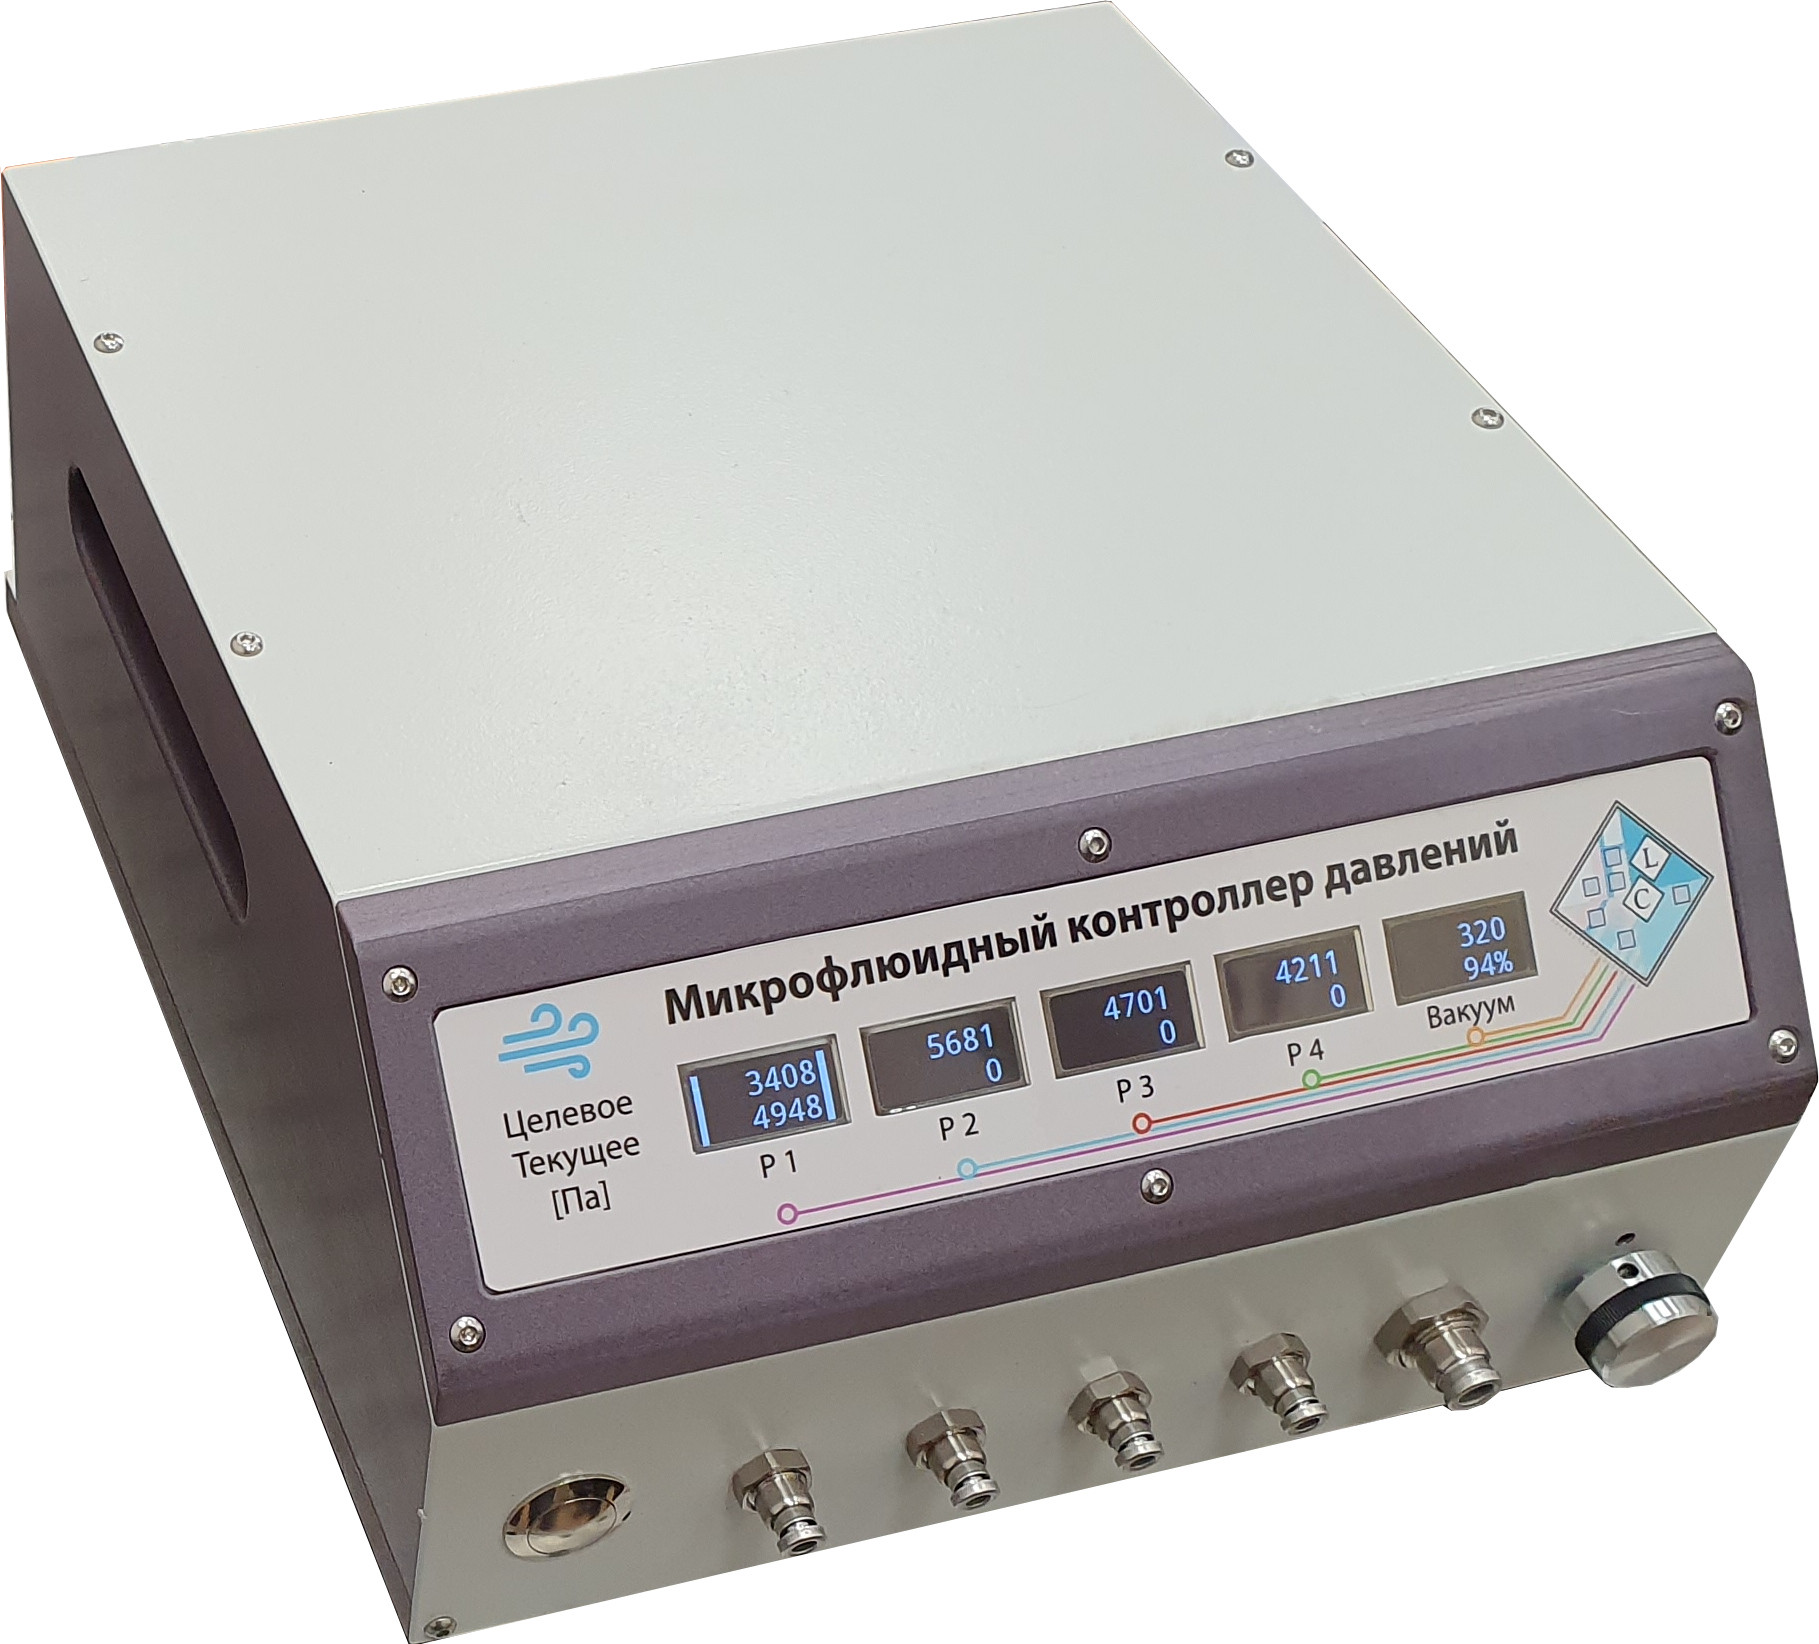
\includegraphics[width=\textwidth]{imgs/device.jpg}
	\caption{Внешний вид микрофлюидного контроллера давлений с пятью дисплеями, четырьмя выходами для положительного давления и одним выходом для вакуумного насоса}
	\label{fig:device}
	\end{center}
\end{figure}


\subsection{Транспортировка}

Вакуумный насос прикреплен к корпуса с помощью силиконовых демпфирующих элементов. Во избежание их повреждения прибор необходимо перевозить в нормальном положении, не переворачивать на бок или вверх ногами. Для транспортировки в багаже необходимо закрепить вакуумный насос, сняв верхнюю крышку прибора\footnote{для этого необходимо использовать специальную шестигранную биту, использование неподходящего инструмента может повредить винты и их будет невозможно выкрутить}.

\subsection{Хранение}

Хранение прибора необходимо производить при условиях, которые не приводят к коррозии металла.

Необходимо разместить заглушки во все пневматические отверстия: одно входное и 5 выходных. Отсутствие заглушек приведет к накоплении микрочастиц, которые могут после начала эксплуатации прибора попасть в микрофлюидный чип и привести к его неисправности. Внутри корпуса на входе пневматической линии прибора установлен фильтр, тем не менее мы рекомендуем выполнять вышеуказанные меры предосторожности и устанавливать заглушку на входной канал во время длительного хранения прибора.


\newpage
\section{Настройка}
\label{setup}

\subsection{Установка приложения}

\href{https://yadi.sk/d/PSVfIjKNqCgW_g}{Ссылка для загрузки приложения}



\subsection{Калибровка}
 


\begin{description}

\item[Панель настройки]
        откройте приложение \textbf{Ветерок}, вызовите справку и найдите кнопку <<калибровка>>.
        
\item[Параметры датчиков]
        коэффициенты A и B ... 
        

\end{description}

%%%%%%%%%%%%%%%%%%%%%%%%%%%%%%%%%%%%%%%%%%%%%%%%%%%%%%%%%%%%%%%%%%%%%%

\newpage
\section{Использование прибора}
\label{usage}

Прибором возможно управления с помощью физической панели управления на передней части прибора или с помощью компьютерного приложения.

\subsection{Панель управления}

\marginlabel{Энкодер:} Прибор оснащен энкодером для ...


\marginlabel{Дисплеи:} Дисплеи информируют о ...



\subsection{Приложение}


\subsubsection{Управление давлением}

\subsubsection{Управление реле}

\subsubsection{Управление вакуумным насосом}



\attention
внимание, если задать такую мощность, которая приведет к остановке насоса, то он может перегреться и выйти из строя. Прибор оснащен защитой от пожара (термопредохранитель прикреплен на двигатель насоса), однако срабатывание системы необратимо без ремонта прибора (замены термопредохранителя).



%%%%%%%%%%%%%%%%%%%%%%%%%%%%%%%%%%%%%%%%%%%%%%%%%%%%%%%%%%%%%%%%%%%%%%
\newpage
\section{Разработка приложения}


\subsection{Исходные коды приложения}

приложение для прибора написано на языке программирования Компонентный Паскаль.

\begin{verbatim}
   MODULE VeterokMain;
   ...
\end{verbatim}

\subsection{Исходные коды прошивки}

%%%%%%%%%%%%%%%%%%%%%%%%%%%%%%%%%%%%%%%%%%%%%%%%%%%%%%%%%%%%%%%%%%%%%%

% \input lay_e2

%%%%%%%%%%%%%%%%%%%%%%%%%%%%%%%%%%%%%%%%%%%%%%%%%%%%%%%%%%%%%%%%%%%%%%

\printindex

\end{document}
